
%\begin{frame}[plain,label=TitlePage]
\begin{frame}[label=TitlePage]
\begin{center}
\textcolor[rgb]{0.2,0.2,0.7}{Correlated states near pressure-induced instabilities} \\
\vspace{0.5em}
{\footnotesize F. M. Grosche} \\
{\footnotesize \em Cavendish Laboratory, Cambridge} \\
\vspace{0.1em}
\end{center}
\vspace{0em}
%\centerline{\multiinclude[<visible@+-| +->][format=pdf,graphics={width=\columnwidth}]{\Figures/FermInstab/QPTScenariosHostGuest2}}
\centerline{ 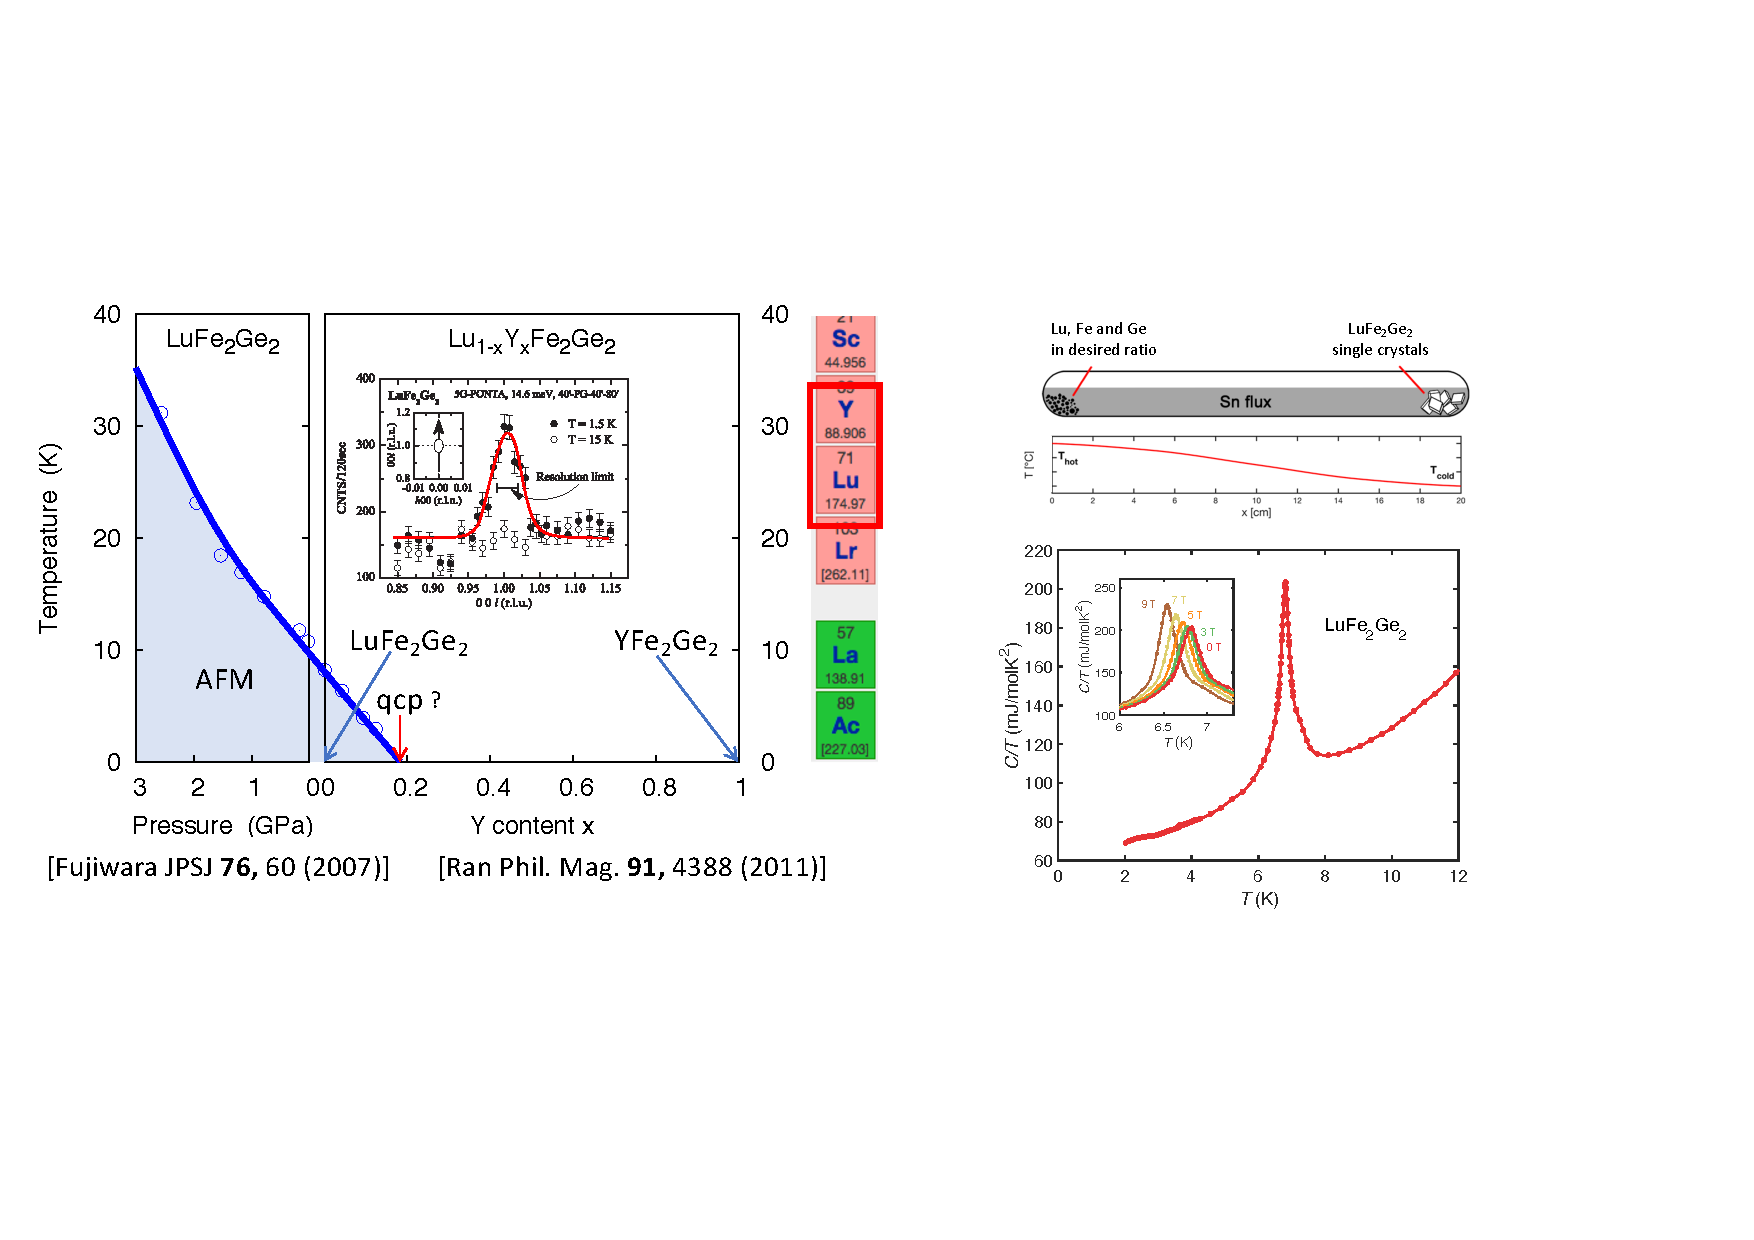
\includegraphics[width=0.95\columnwidth]{IntroPicture}}

% \vspace*{\fill}
% \centerline{\makebox[\linewidth]{\rule{0.85\textwidth}{0.4pt}}}
% \centerline{\scriptsize S. Goh {\it et al.} Phys. Rev. Lett. {\bf 114,} 097002 (2015)}
% \centerline{\scriptsize S. Friedemann {\it et al.} Sci. Rep. {\bf 6,} 416 (2016)}

\begin{itemize}
%\item Quantum effects at accessible temperatures
\item Tunability of correlated systems
\item Plenty of room in material space
%\item Instrumentation 
%\item Current research topics
\item Quantum functional materials
\end{itemize}


% \end{columns}
% \onslide+<2->
% \begin{center} 
% Thermal de Broglie wavelength $\lambda \propto 1/\sqrt{m T}$
% \end{center}

\vspace{0.3em}
\visible<2->{
\centerline{Quantum degeneracy temperature for electrons in metals: }
\[
T_F \sim ~\frac{\text{(density)}^{2/3}}{\text{mass}} \simeq 10,000 ~\text{degrees}
\]
}


\end{frame}


%%%%%%%%%%%%%%%%%%%%%%%%%%%%%%%%%%%%%%%%%%%%%%%%%%%%%%%%%%%%%%%%%%%%%%

\begin{frame}[plain,label=Conc]
\frametitle {Key contributors}
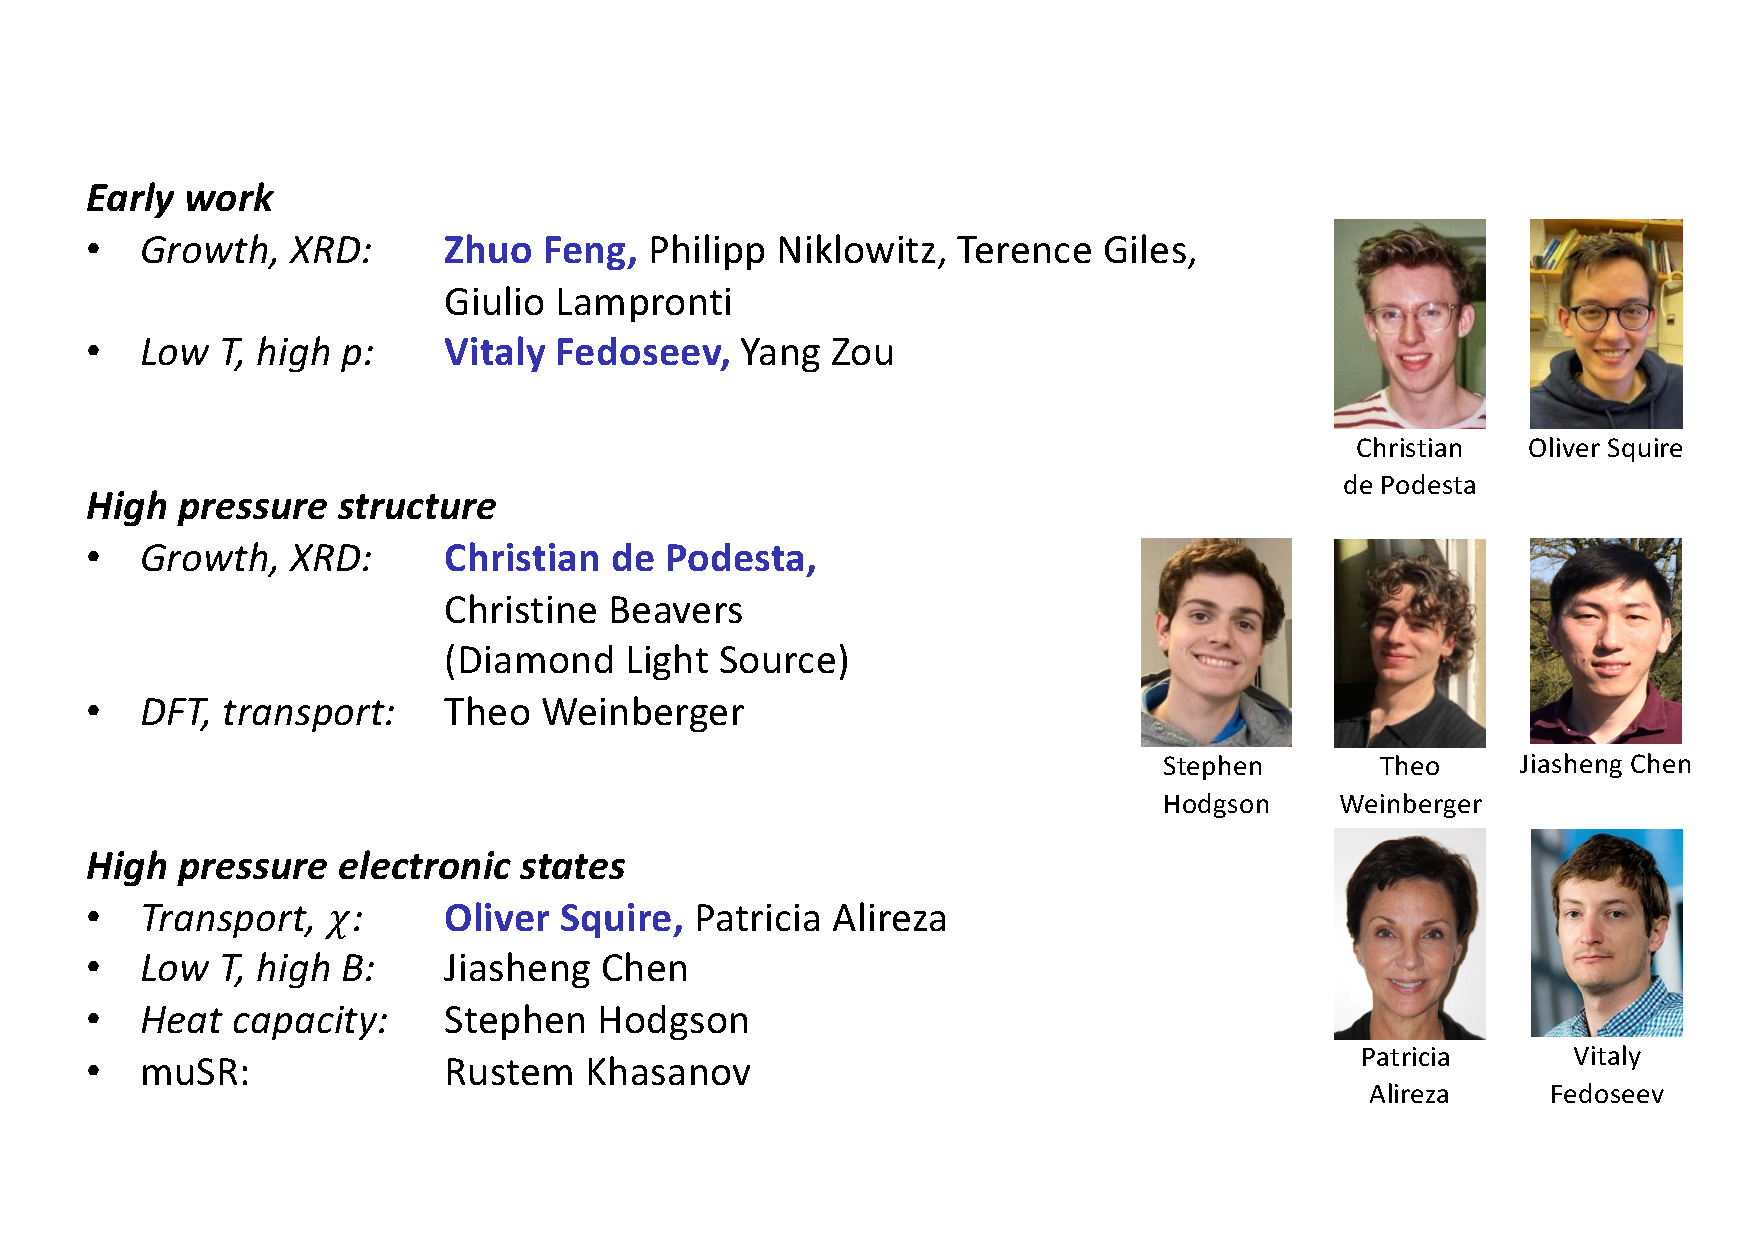
\includegraphics[width=1.25\textwidth]{GroupList}
\end{frame}

%%%%%%%%%%%%%%%%%%%%%%%%%%%%%%%%%%%%%%%%%%%%%%%%%%%%%%%%%%%%%%%%%%%%%%

\begin{frame}[plain,label=Conc]
\frametitle {Key contributors}
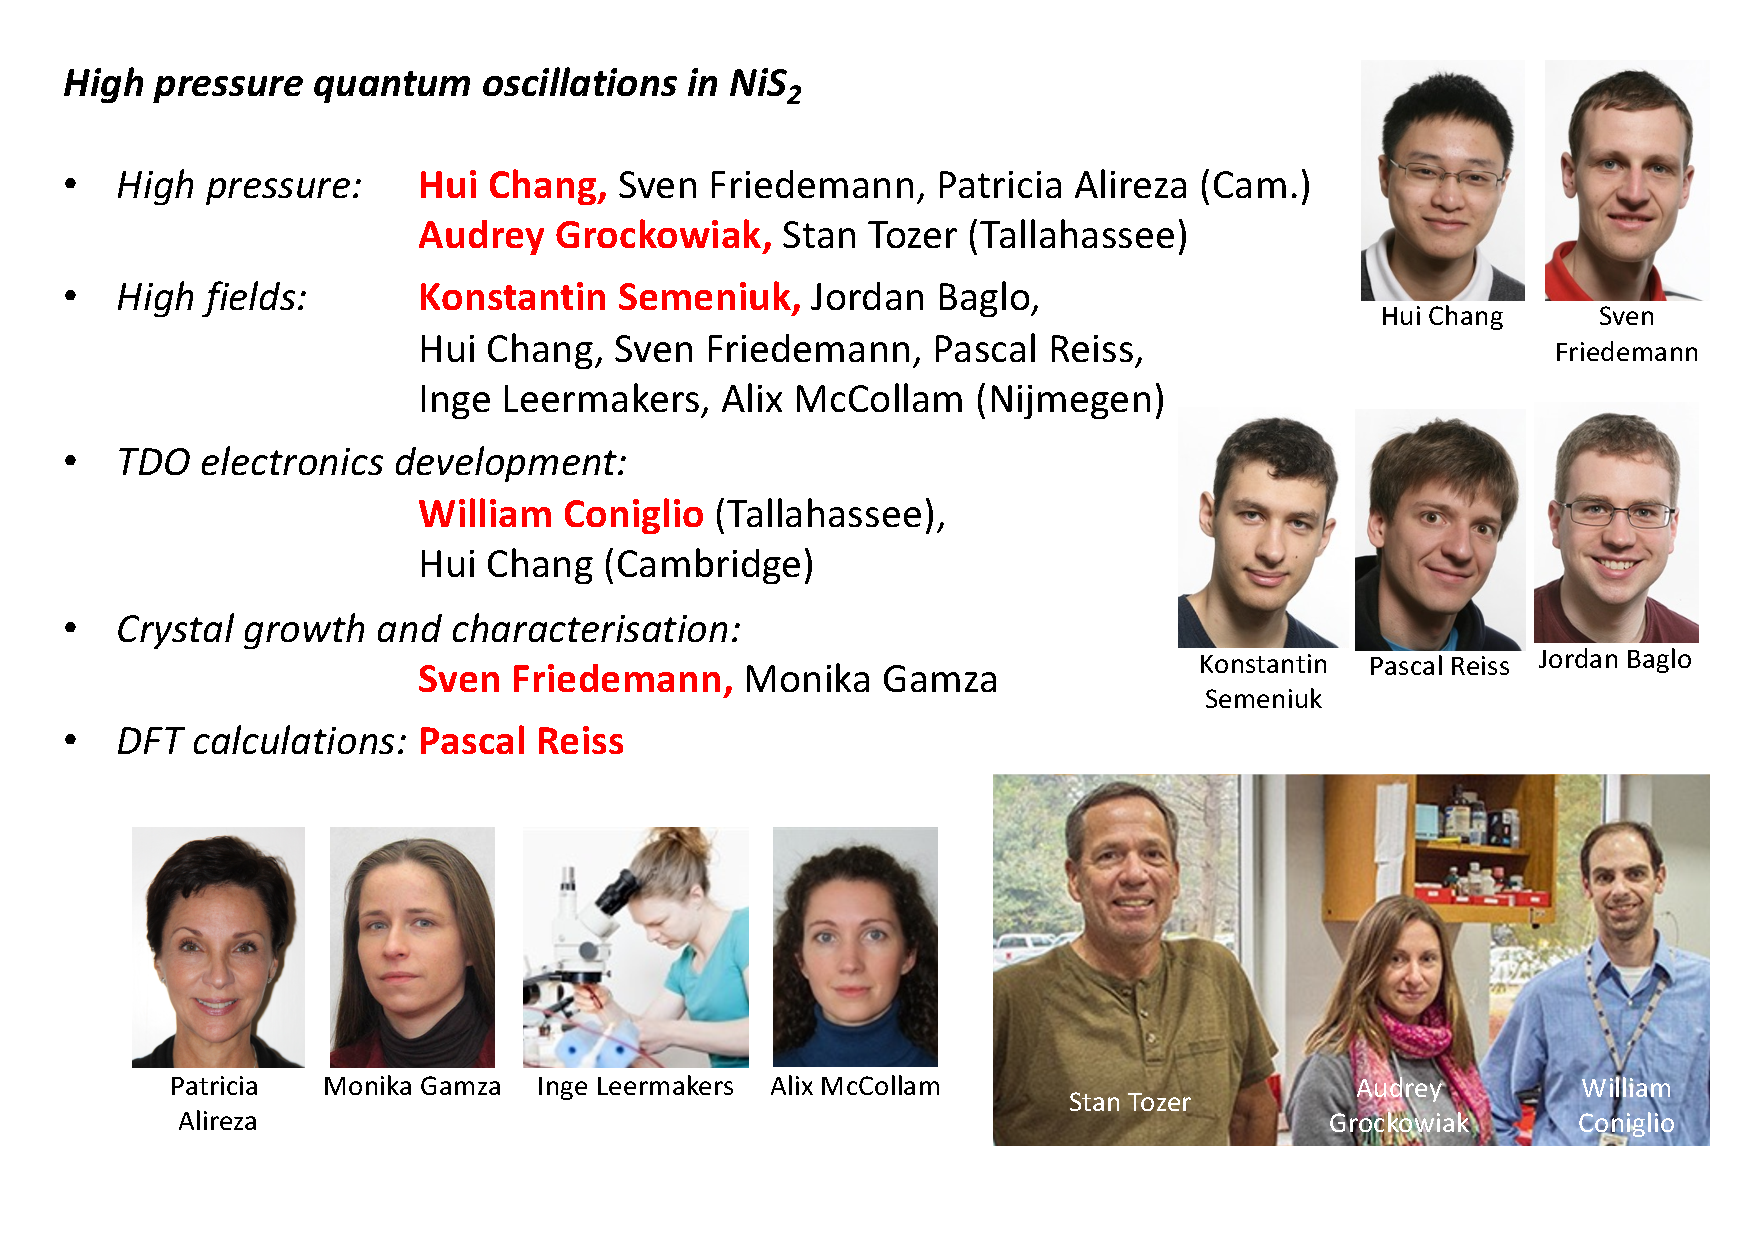
\includegraphics[width=1.25\textwidth]{GroupListNiS2}
%{\scriptsize
% \hl{YFe$_2$Ge$_2$}
% \begin{itemize}
% %\setlength{\baselineskip}{1.4em}
% \item{Samples:} \hfill
% \hl{Jiasheng Chen,} Zhuo Feng 
% %% \\ \raggedleft{Geetha Balakrishnan  (Warwick)}

% \item{Measurements:} \hfill  \hl{Konstantin Semeniuk,} Phil Brown %, Yang Zou, Peter Logg
% % \item{Low-$T$ magnetic susceptibility:} \hfill Christopher Harrison, \\
% %   \raggedleft{\hl{Philipp Niklowitz} (RHUL), Jordan Baglo}

% %\item{Band structure calculations:} \hfill {Pascal Reiss}
% \end{itemize}

% \hl{R$_3$T$_4$Sn$_{13}$}
% \begin{itemize}
% \setlength{\baselineskip}{1.4em}
% \item{Crystals:} \hfill
% J. Yang, B. Chen, \raggedleft{\hl{K. Yoshimura} (Kyoto and Hangzhou)}

% \item{High pressure:} \hfill
% \hl{Swee Goh,} Lina Klintberg
% \item{X-ray diffraction:} \hfill \hl{Paul Saines} 
% \end{itemize}

% \vspace{1em}


%  \hl{Bi-III}
% \begin{itemize}
% \item{Measurements:} \hfill 
% \hl {Phil Brown,} Konstantin Semeniuk, Alex Vasiljkovic

% \item{DFT calculations} \hfill
% \hl{Bartomeu Monserrat,} Chris Pickard, Diandian Wang
% \end{itemize}

% \vspace{1em}

% \hl{Fermi surface of pressure-metallised NiS$_2$}
% \begin{itemize}
% \item{Crystals:} \hfill \hl{Sven Friedemann,} Monika Gamza
% \item{High $p$ quantum oscillations:} \hfill \hl{Hui Chang, Sven Friedemann,} \\
% \raggedleft {Konstantin Semeniuk,} Jordan Baglo
% \item {High field measurements:} \hfill \hl{A. Grockowiak,} W. Coniglio, S. Tozer
%   (Tallahassee), \\ \raggedleft{I. Leermakers, A.
%   McCollam (Nijmegen)}

% \item{DFT calculations:} \hfill
% Pascal Reiss
%\end{itemize}

% \hl{NbFe$_2$}
% \begin{itemize}
% \setlength{\baselineskip}{1.4em}
% \item{Single crystals:} \hfill
% \hl{Will Duncan,} Andreas Neubauer,  \\ \raggedleft{Christian Pfleiderer
%   (RHUL, Munich)}


% % \item{$\mu$SR:} \hfill \hl{Daniela Rauch,} Stefan S\"ullow, \\
% % \raggedleft{M. Kraken, H. Luetkens, Jochen Litterst (Braunschweig)}

% % \item{ESR, dilatometry:} \hfill Thomas Bauer, \\ 
% % \raggedleft{Tobias F\"orster,  \hl{Manuel Brando} (Dresden)}

% \item{Magnetometry, resistivity:} \hfill
% \hl{Sven Friedemann,} Max Hirschberger
%   (Cambridge)

% \item{Neutron scattering:} \hfill
% \hl{Philipp Niklowitz,} Marijn Lucas (RHUL), Max Hirschberger, \\ 
% \raggedleft{Astrid
%   Schneidewind, Petr Cermak, Enrico Faulhaber (Munich)}
% \end{itemize}

% \hl{CeSb$_2$}
% \begin{itemize}
% \item{Crystals:} \hfill \hl{Zhuo Feng,} Takao
%   Ebihara (Shizuoka)

% \item{Measurements:} \hfill 
% \hl {Vitaly Fedoseev}, Yang Zou

% \item{High-$p$ x-rays:} \hfill
% \hl{Philipp Niklowitz,} Terence Giles, \raggedleft{Heribert Wilhelm}
% \end{itemize}

%\vspace{1em}


% \rule{\textwidth}{0.4pt}
% \begin{itemize}

% % \item{X-ray diffraction:} \hfill
% % Giulio Lampronti, Paul Saines 

% \item{High pressure training and support:} \hfill
% Patricia Alireza

% \item{Discussions, motivation and ideas:} \hfill
% \hl{Gil Lonzarich} % \\ \raggedleft{Philipp Niklowitz (RHUL)}

% \end{itemize}

%}

% \item{Discussions, motivation and ideas:} \hfill
% \hl{Gil Lonzarich,} \\ \raggedleft{Christoph Geibel, Manuel Brando, Sven Friedemann}

% \item{Neutron scattering:} \hfill
% \hl{Philipp Niklowitz (RHUL),} \\ 
% \raggedleft{Max Hirschberger, Astrid
%   Schneidewind, Enrico Faulhaber (Munich)}
%\end{itemize}


% \item{SQUID anvil cells, mini-coils:} \hfill
% \hl{Patricia Alireza}



% \item{High field measurements:} \hfill
% Mike Sutherland
%
%\begin{textblock}{4}(4, -5.2)
%\visible<2->{
%\begin{beamercolorbox}{postit}
%\begin{center}
%\textcolor{red}{Probably won't \\ get this far...}
%\end{center}
%\end{beamercolorbox}
%}
%\end{textblock}

\end{frame}







%%% Local Variables: 
%%% mode: latex
%%% TeX-master: "GroTalk.ho"
%%% End: 


%%%%%%%%%%%%%%%%%%%%%%%%%%%%%%%%%%%%%%%%%%%%%%%%%%%%%%%%%%%%%%%%%%%%%
\begin{frame}[plain,label=TitlePage]
\frametitle{Quantum Matter group}
\hspace{5em}\includegraphics[width=1.2\columnwidth]{\Figures/GroupAdvertising/GruppenBilder2018}

\end{frame}






%%% Local Variables: 
%%% mode: latex
%%% TeX-master: "GroTalk"
%%% End: 
